\section{Rastreamento dos Usuários}

	O rastreamento é fundamental para o funcionamento correto do Sistema TRUE uma
	vez que é responsável por rastrear os usuários no ambiente, determinar a sua localização
	física em relação ao sensor \textit{Kinect} e gerenciar suas identidades.
	Portanto, foi realizado uma série de testes funcionais para avaliar o modulo de
	rastreamento do Sistema TRUE.
		
	\begin{figure}[htb]
		\begin{center}
 			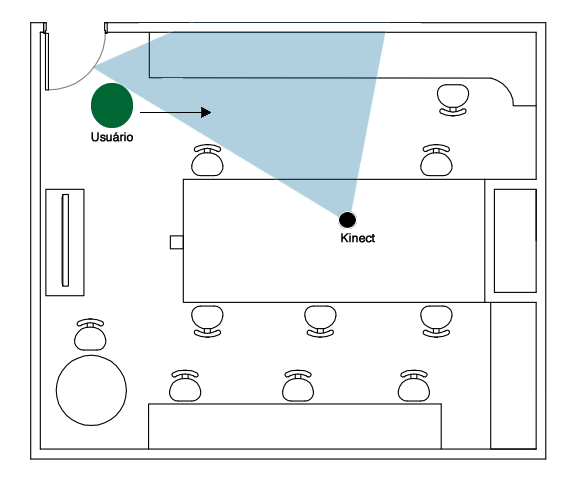
\includegraphics[width=0.4\textwidth]{figuras/4.ProblemaEProposta/laico-teste-deteccao.png}
 		\end{center}
 		\caption{Demostração do teste de detecção dentro do \textit{SmartSpace}
 		Laico.}
		\label{fig:laico-teste-deteccao}
	\end{figure}		
	
	Os primeiros testes realizados tiveram como objetivo verificar a eficiência da
	detecção de novos usuários no ambiente. Os testes foram feitos simulando a
	entrada de um usuário na cena e analisando o momento em que o mesmo era
	detectado. Esse teste foi executado no Laico e a posição do sensor e a
	trajetória do usuário é apresentado na Figura~\ref{fig:laico-teste-deteccao}. Em
	todos os testes o usuário era detectado antes mesmo de entrar na área de visão
	do sistema por completo, como mostrado na Figura~\ref{fig:testes_deteccao}.
	
	\begin{figure}[htb]
		\begin{center}
				\subfloat[] {
					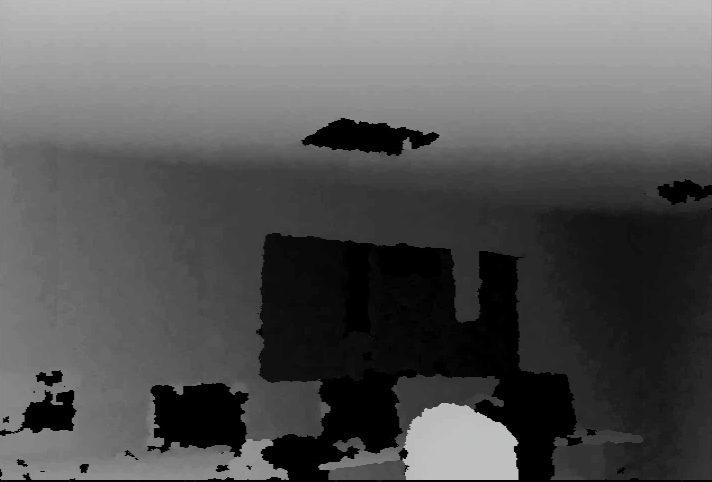
\includegraphics[width=0.25\textwidth]{figuras/5.Testes/deteccao/1.png}}
				\subfloat[] {
					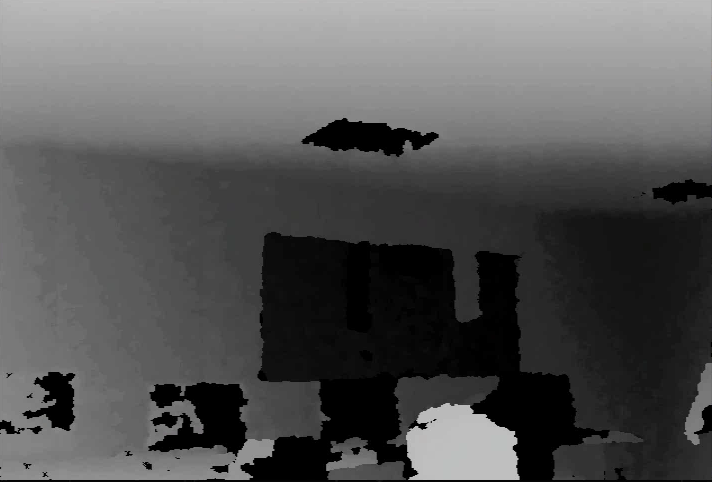
\includegraphics[width=0.25\textwidth]{figuras/5.Testes/deteccao/2.png}}
				\subfloat[] {
					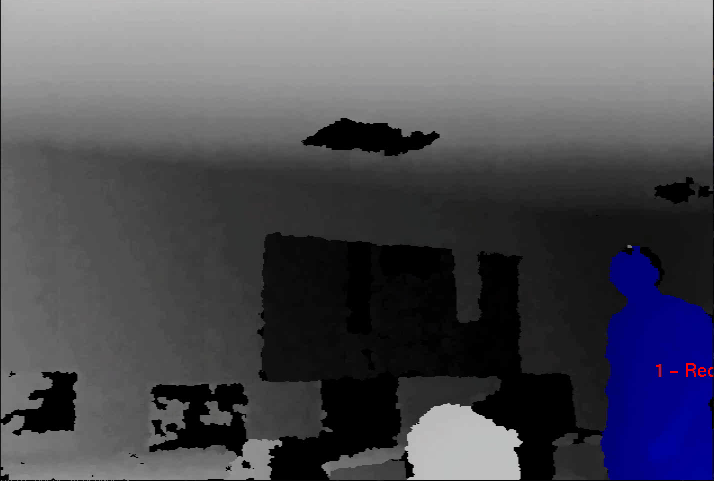
\includegraphics[width=0.25\textwidth]{figuras/5.Testes/deteccao/3.png}}
				\subfloat[] {
					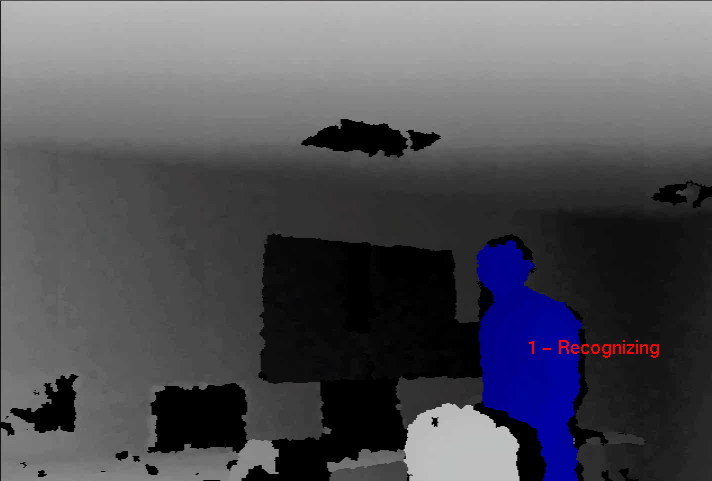
\includegraphics[width=0.25\textwidth]{figuras/5.Testes/deteccao/4.png}}
		\end{center}
		\caption{Momento em que um novo usuário foi detectado pelo Sistema TRUE.}
		\label{fig:testes_deteccao}
	\end{figure}
		
	Também foram realizados testes com o objetivo de verificar a oclusão no
	rastreamento. Foi testado o caso em que um usuário oculta propositalmente outro
	já rastreado. Nesta situação, caso o usuário rastreado continuasse oculto, o
	sistema o determinava como perdido. Por outro lado, nos casos de oclusão
	parcial, o sistema se mostrou robusto como pode ser observado na
	Figura~\ref{fig:testes_oclusao_sucesso}, onde o usuário apresentado na cor verde
	está parcialmente oculto pelo usuário na cor azul. Nos testes foi simulada
	também a situação de oclusão momentânea, ou seja, um usuário em movimento oculta
	outro por um curto período de tempo em razão da sua movimentação. Nestes casos,
	o sistema TRUE perde o usuário rastreado, mas rapidamente é capaz de detectá-lo
	novamente, como mostrado na sequência de imagens da
	Figura~\ref{fig:testes_oclusao}. A oclusão era um problema esperado uma vez que
	o Sistema TRUE utiliza somente um sensor \textit{Kinect} como dispositivo de
	entrada.
			
	\begin{figure}[htb]
		\begin{center}
			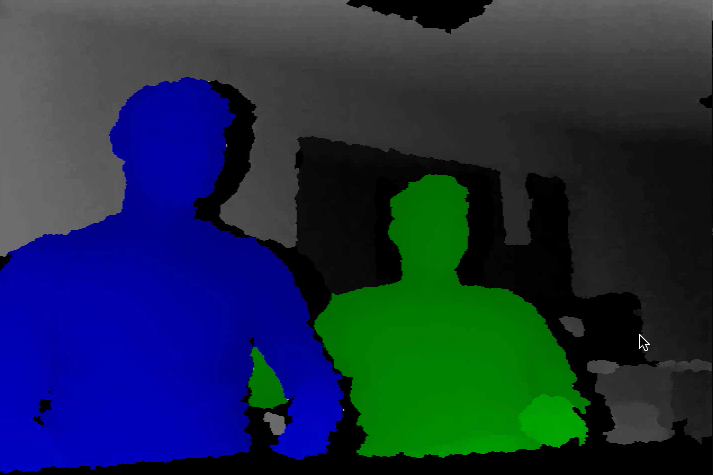
\includegraphics[width=0.75\textwidth]{figuras/5.Testes/oclusao/oclusao_corretamente.png}
		\end{center}
		\caption{Oclusão parcial de usuário rastreado.}
		\label{fig:testes_oclusao_sucesso}
	\end{figure}

	\begin{figure}[htb]
	\begin{center}
			\subfloat[] {
				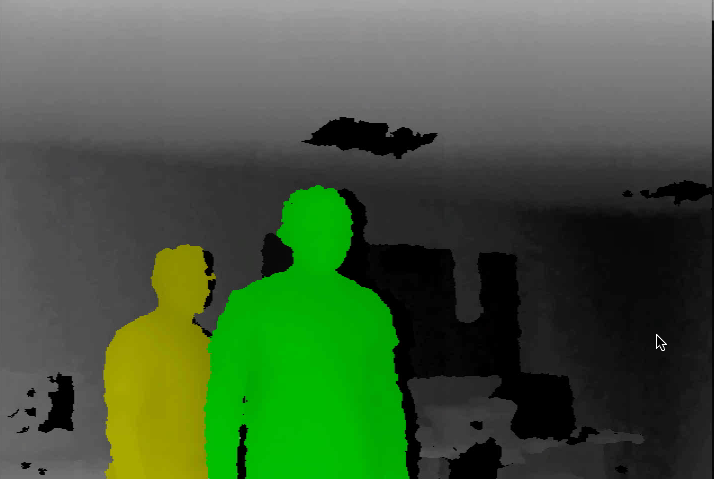
\includegraphics[width=0.19\textwidth]{figuras/5.Testes/oclusao/1.png}}
			\subfloat[] {
				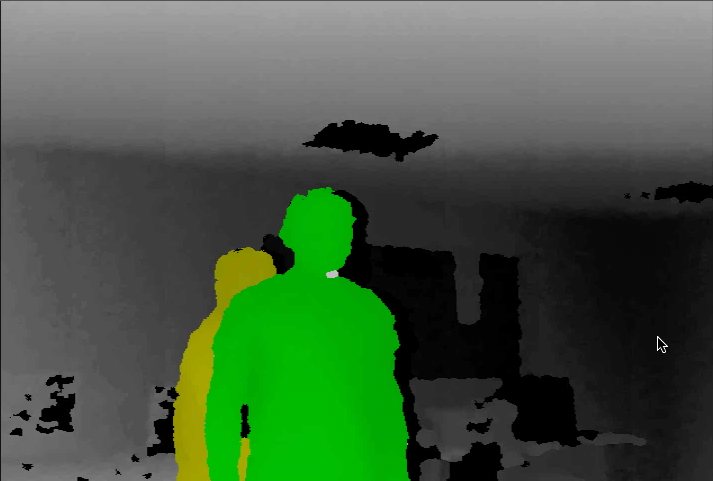
\includegraphics[width=0.19\textwidth]{figuras/5.Testes/oclusao/2.png}}
			\subfloat[] {
				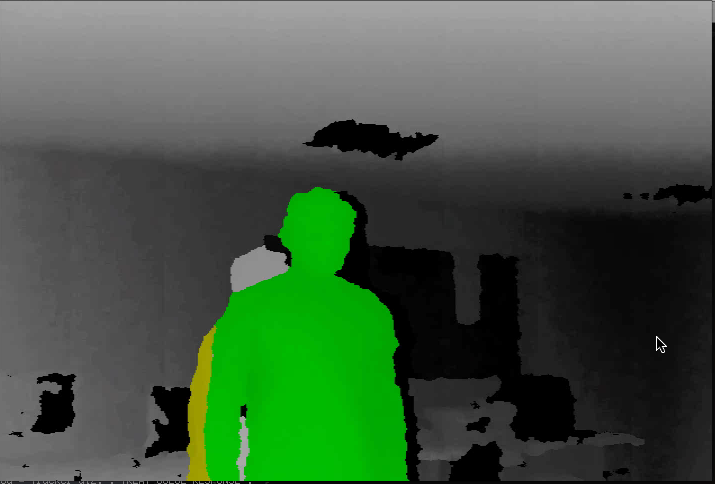
\includegraphics[width=0.19\textwidth]{figuras/5.Testes/oclusao/3.png}}
			\subfloat[] {
				\label{fig:testes_oclusao_ocluso}
				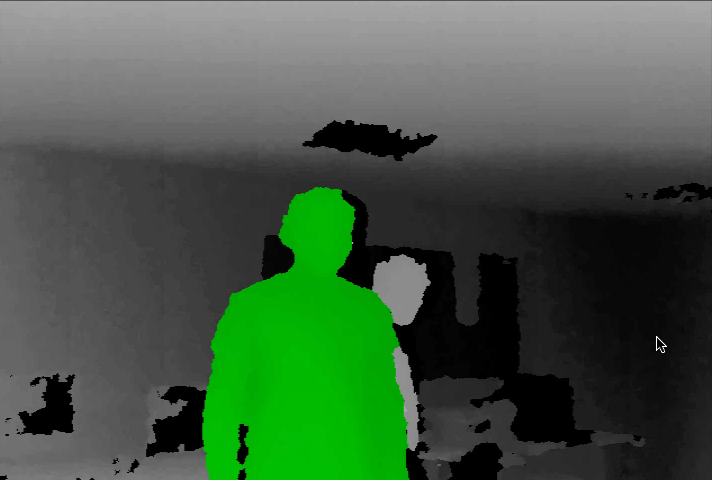
\includegraphics[width=0.19\textwidth]{figuras/5.Testes/oclusao/4.png}}
			\subfloat[] {
				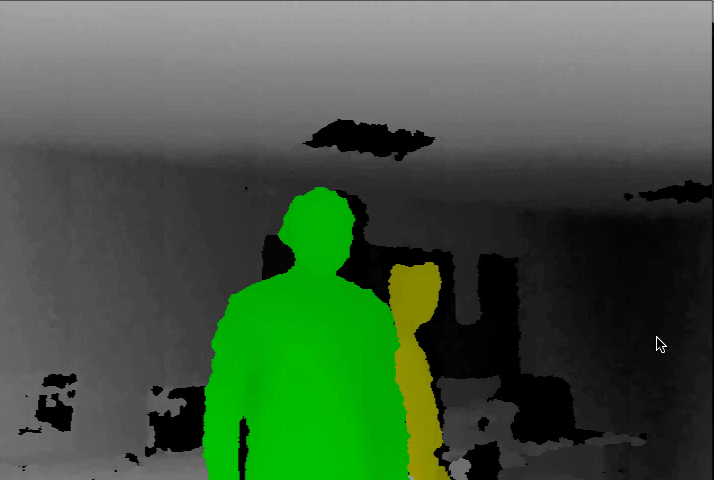
\includegraphics[width=0.19\textwidth]{figuras/5.Testes/oclusao/5.png}}
		\end{center}
		\caption{Oclusão de usuários.}
		\label{fig:testes_oclusao}
	\end{figure}

	Dado que o \textit{Kinect} tem um ângulo de 57º e foi comprovado em testes
	que o alcance maximo é de 4057 milímetros (Seção~\ref{sec:testes-localizacao})
	elaboramos o seguinte teste. A uma distância de aproximadamente 4 metros do
	sensor foram dispostos, ombro a ombro, o maximo de usuários sem que
	haja oclusão ou interferência. Neste teste conseguimos que até 5 usuários
	fossem rastreados como é possível ver na Figura~\ref{fig:max-pessoas}.

% 	Com relação a abrangência do campo de visão do Sistema TRUE, tendo em vista que
% 	ele utiliza o sensor \textit{Kinect} cujo campo de visão horizontal é de 57º e
% 	cujos testes mostraram que tem alcance maximo de 4,057 metros
% 	(Seção~\ref{sec:testes-localizacao}), é possível até uma distância de,
% 	aproximadamente, 4 metros do sensor, ter até 5 usuários no campo de visão sem
% 	que haja oclusão de pessoas (Figura~\ref{fig:max-pessoas}).
	
	% TODO: jogar isso aqui.
% 	Através deste teste, também foi possível obter a distância máxima e mínima que o usuário
% deve estar do Kinect para que o sistema consiga rastrea-lo e estimar sua localização. A distância
% mínima é de 48, 3cm e a máxima de 4, 057m.
	

	\begin{figure}[htb]
		\begin{center}
			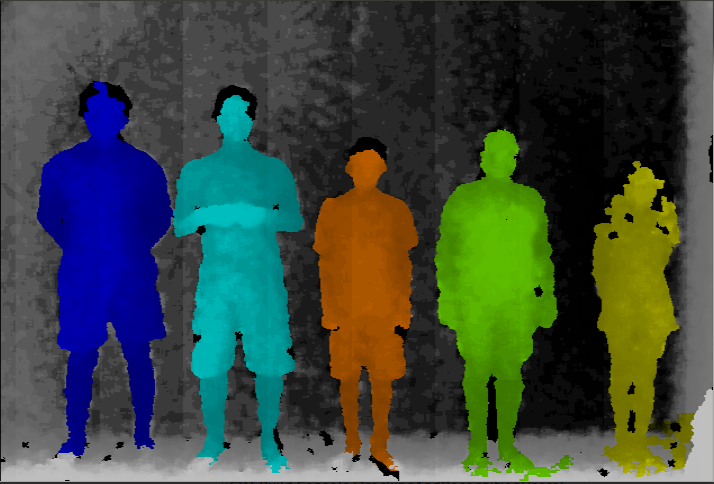
\includegraphics[width=0.4\textwidth]{figuras/5.Testes/oclusao/max-pessoas.png}
		\end{center}
		\caption{Usuários posicionados lado a lado a uma distância de 4 metros do
		sensor \textit{Kinect}.}
		\label{fig:max-pessoas}
	\end{figure}
		
	Durante os testes realizados com rastreamento foi observado alguns problemas
	quando o usuário rastreado interagia com objetos do ambiente ou com outros
	usuários. Na grande maioria das vezes em que o usuário interagiu com objetos, o
	Sistema TRUE considerou o objeto como sendo parte do usuário, conforme
	exemplificado na Figura~\ref{fig:testes_relacionamento_com_objetos}. Entretando,
	esta situação não prejudicou a eficiência do sistema. Por outro lado, os
	problemas com interação entre usuários foram mais raros, porém tiveram impacto
	maior. Tais problemas consistem em ``interferências'' que ocorreram em algumas
	situações de contato entre dois ou mais usuários, conforme exemplifica a
	Figura~\ref{fig:testes_relacionamento_com_usuarios}.
	
	\begin{figure}[htb]
		\begin{center}
			\subfloat[] {
				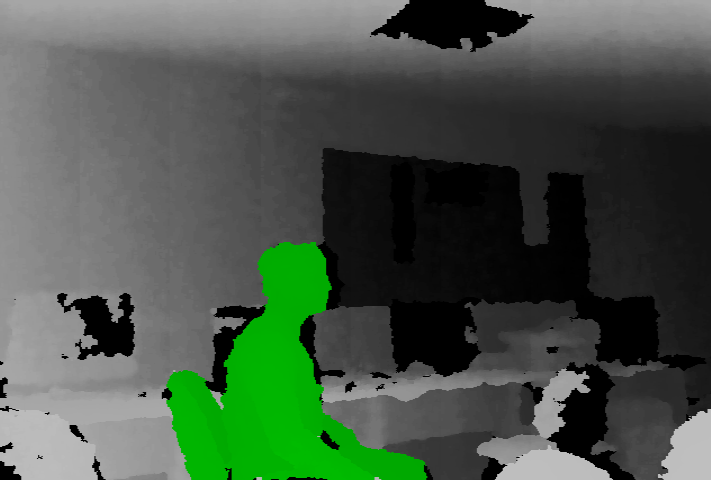
\includegraphics[width=0.37\textwidth]{figuras/5.Testes/relacionamento_com_objetos/1.png}}
			\subfloat[] {
				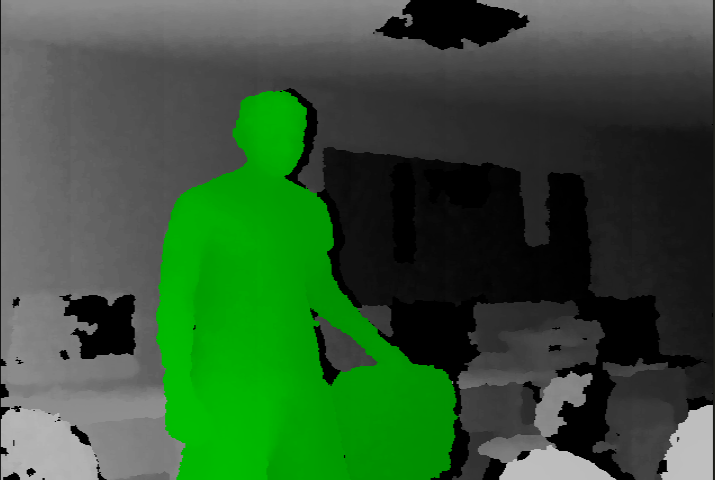
\includegraphics[width=0.37\textwidth]{figuras/5.Testes/relacionamento_com_objetos/2.png}}
		\end{center}
		\caption{Usuário sendo rastreado em conjunto com o objeto que interage.}
		\label{fig:testes_relacionamento_com_objetos}
	\end{figure}
		
	\begin{figure}[htb]
		\begin{center}
			\subfloat[] {
				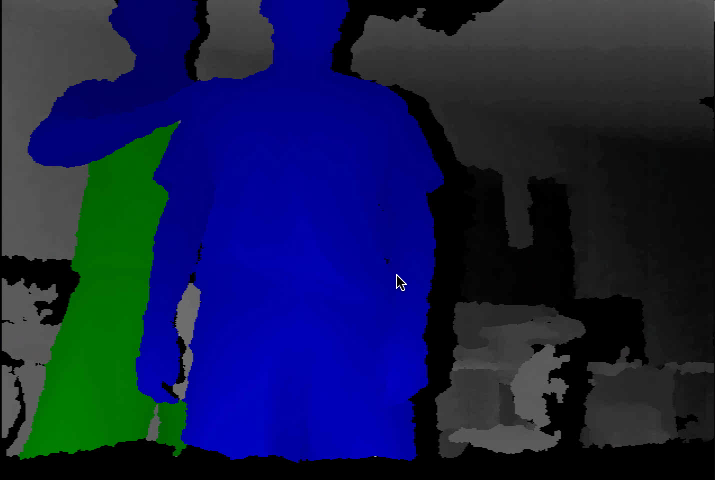
\includegraphics[width=0.32\textwidth]{figuras/5.Testes/relacionamento_com_pessoas/1.png}}
			\subfloat[] {
				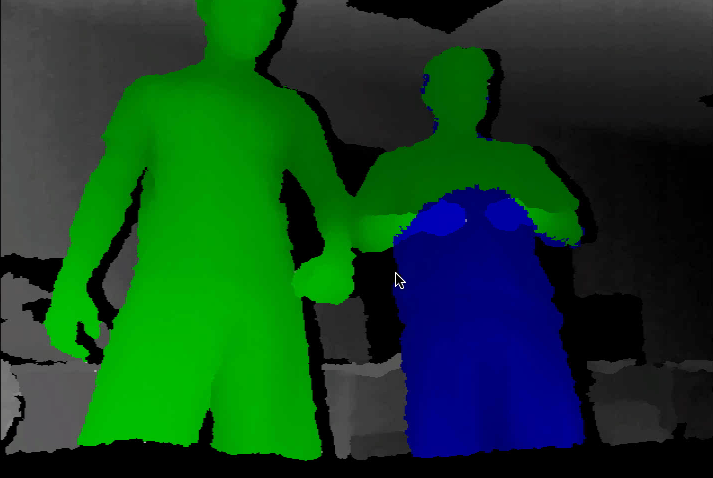
\includegraphics[width=0.32\textwidth]{figuras/5.Testes/relacionamento_com_pessoas/2.png}}
			\subfloat[] {
				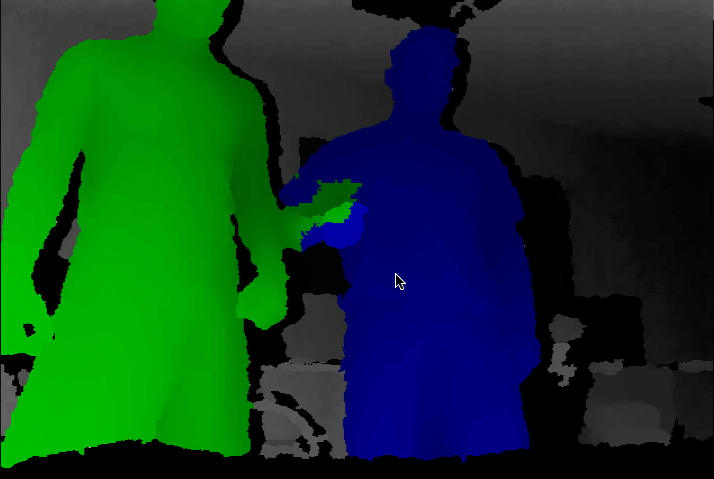
\includegraphics[width=0.32\textwidth]{figuras/5.Testes/relacionamento_com_pessoas/3.png}}
		\end{center}
		\caption{Usuários sofrendo interferência de outros ao seu redor.}
		\label{fig:testes_relacionamento_com_usuarios}
	\end{figure}

	Apesar dos problemas relatados, o rastreamento conseguiu, na maioria dos testes,
	atender às necessidades rastreando os diversos usuários no ambiente em suas
	atividades diárias, como mostrado na Figura~\ref{fig:varios-usuarios-ambiente}.

	\begin{figure}[htb]
		\begin{center}
			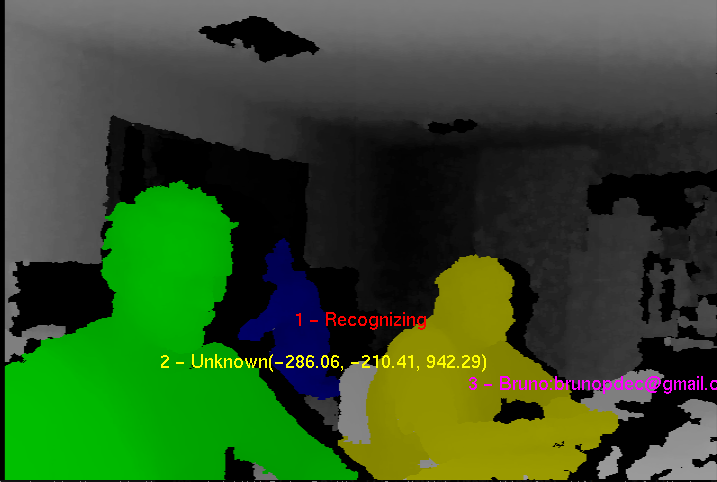
\includegraphics[scale=0.5]{figuras/5.Testes/oclusao/usuarios-rastreados.png}
		\end{center}
		\caption{Usuários do LAICO rastreados pelo Sistema TRUE.}
		\label{fig:varios-usuarios-ambiente}
	\end{figure}	